\section{Spatial and drones}\label{spatial-and-drones}

\begin{frame}{An exciting target}

\begin{itemize}
\tightlist
\item
  Exciting demo for spatial \(\Rightarrow\) Answer to why spatial, and
  what can spatial do
\item
  Intellectually stimulating \(\Rightarrow\) Lots of research on the
  subject
\end{itemize}

\end{frame}

\begin{frame}{Full of potential}

Air is still very much an uncharted territory:

\begin{itemize}
\tightlist
\item
  Surveillance
\item
  Search and rescue
\item
  Logistic inside warehouses
\item
  Transport of materials or documents
\item
  Monitoring (crops, protection of species in danger)
\end{itemize}

\end{frame}

\section{A constrained problem}\label{a-constrained-problem}

\begin{frame}{Energy bound}

Improved efficiency \(\Rightarrow\) Extended flight time

\begin{itemize}
\tightlist
\item
  Hovering rule of thumb: \textbf{\textasciitilde{}150W/Kg}
\item
  A drone like the AF450 from our lab \textbf{\textasciitilde{}100W}
\item
  His FMU (Flight Management Unit), a Pixhawk:
  \textbf{\textasciitilde{}1-2W}
\item
  Jetson TX2, the latest embedded CUDA board from NVIDIA consumes
  around: \textbf{\textasciitilde{}8W}
\end{itemize}

\end{frame}

\begin{frame}{Latency bound}

\textbf{SLAM} (Software localization and mapping) is critical for
\textbf{motion planning} and \textbf{motion control}.

A critical subproblem of \textbf{SLAM} is \textbf{POSE} (position
estimation)

\end{frame}

\begin{frame}{}

\[\hat{x_t} = f(x_{t-1}, O_t)\]

\begin{itemize}
\tightlist
\item
  \(x_t\) is the state of the drone (including position, attitude
  (orientation), velocity, etc \ldots{}) at time t
\item
  \(\hat{x}\) is the estimation of that state
\item
  \(O_t\) is the observation of the universe by the drone at time t
\item
  \(f\) is the SLAM prediction algorithm
\end{itemize}

\end{frame}

\begin{frame}{}

Latency = \(\Delta t\)

\(=\) Max(f time, O sample rate)

Reduce f computation time closer to O sample rate.

\end{frame}

\begin{frame}{}

Reduced latency result in more accurate \(\hat{x_t}\):

\begin{itemize}
\tightlist
\item
  Smoother control \(\Rightarrow\) Less jiggering + ``agile'' drone
\item
  Better sync between planning and control
\item
  Better collision avoidance \(\Rightarrow\) safer for the drone and its
  surrounding.
\end{itemize}

\end{frame}

\begin{frame}{Performance bound}

Currently, heavy tasks are usually done:

\begin{itemize}
\tightlist
\item
  On a companion computer on the ground
\item
  Sometimes, offline (after the flight) from the data gathered
\end{itemize}

Preferable or critical to do them \textbf{onboard} and \textbf{online}

\end{frame}

\begin{frame}{The vision}

\textbf{Accelerating hardware! }

\emph{(A plasticine in every drone)}

\begin{itemize}
\tightlist
\item
  Efficient
\item
  Low-latency
\item
  Performant
\end{itemize}

Focus on \textbf{FPGA} and likely the \textbf{OcPoc} from aerotenna
which include a \textbf{cyclone V}.

\end{frame}

\begin{frame}{}

\begin{itemize}
\tightlist
\item
  Plasticine: An hardware architecture made by us for spatial
\item
  FPGA: A common reprogrammable hardware achitecture targetable by
  spatial
\item
  Spatial: the compiler from DSL to spatial hardware architecture
  program
\end{itemize}

\end{frame}

\section{Sensor fusion}\label{sensor-fusion}

\begin{frame}{Sensor fusion}

Sensor fusion is the fusion of the data from different sensor to get
accurate estimator of one state.

\begin{itemize}
\tightlist
\item
  Dual GPS
\item
  accelerometer + gyroscope for attitude
\item
  LIDAR + IMU
\end{itemize}

Sensor fusion can be achieved through the combination of filtered
signals.

\end{frame}

\begin{frame}{}

\begin{figure}
\centering
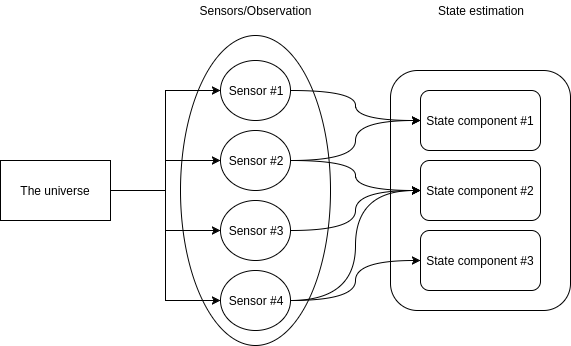
\includegraphics{fusion.png}
\caption{Sensor fusion}
\end{figure}

\end{frame}

\begin{frame}{Sensor Filters}

There is two main filters for POSE:

\begin{itemize}
\tightlist
\item
  Complementary filters
\item
  Kalman filters
\end{itemize}

\end{frame}

\begin{frame}{Complementary filters}

Complementary filters come from the complentarity of a HPF and a LPF
applied to different sensors

For instance, retrieving the attitude/orientation from the gyroscope +
accelerometer

\end{frame}

\begin{frame}{}

\begin{figure}
\centering
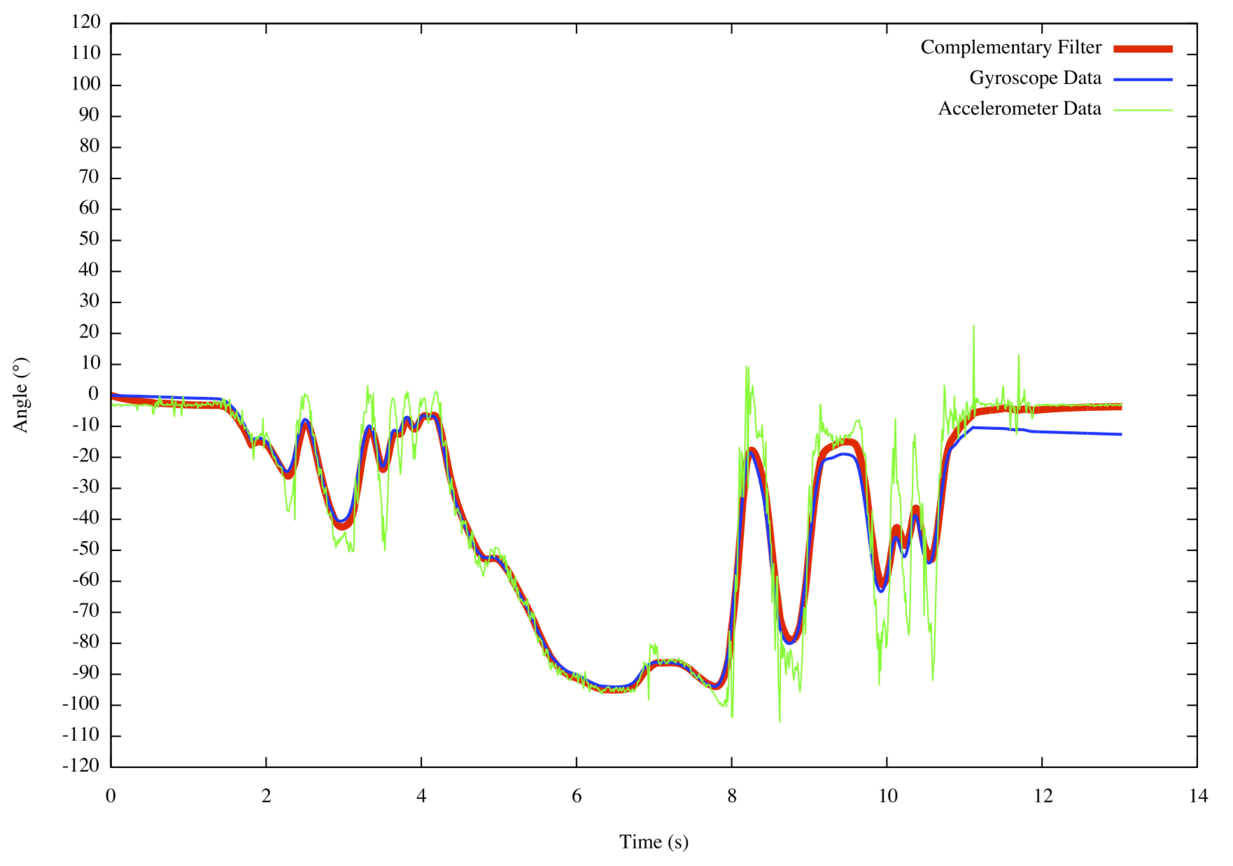
\includegraphics{cf.png}
\caption{orientation}
\end{figure}

\end{frame}

\begin{frame}{Accelerometer}

accelerometer (through g acceleration) no drift but high-variance at
high frequency (vibrations, other forces)

Accurate in the long-term: \textbf{Low-pass filter}

\begin{figure}
\centering
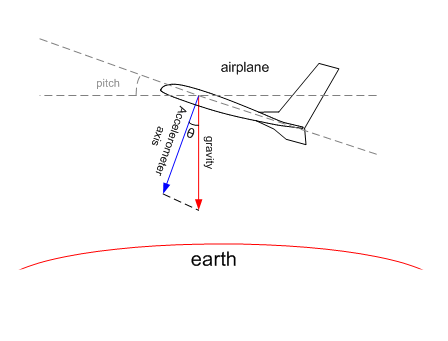
\includegraphics{accelero.png}
\caption{Accelerometer}
\end{figure}

\end{frame}

\begin{frame}{Gyroscope}

gyroscope drift (because of integral over numerical error accumulate)

Accurate in the short term: \textbf{High-pass filter}

\begin{figure}
\centering
\includegraphics{gyro.gif}
\caption{Gyroscope}
\end{figure}

\end{frame}

\begin{frame}{Drift}

\begin{itemize}
\tightlist
\item
  Why does the gyro drift ? Because of the nature of an integration over
  a gaussian.
\item
  Even if the noise (sensor noise + floating point error) has no bias,
  it accumulates errors over time.
\item
  \[Z \sim N(\mu_X + \mu_Y, \sigma_X^2 + \sigma_Y^2)\]
\item
  For better intuition, see Wiener process \(Var(W_t) = t\)
\end{itemize}

\end{frame}

\begin{frame}{Kalman Filters}

Also called linear quadratic estimation (LQE)

Estimate the joint state random variables (like position) conditonned on
a a series of noisy observation (from the sensors).

\end{frame}

\begin{frame}{}

Basic principle, true state \(x_t\) is a linear noisy process:

\[\mathbf{x}_t = \mathbf{F}_t \mathbf{x}_{t-1} + \mathbf{B}_t \mathbf{u}_t + \mathbf{w}_t \]

\begin{itemize}
\tightlist
\item
  \(\mathbf{F}_t\) the state transition model
\item
  \(\mathbf{B}_t\) the control-input model
\item
  \(\mathbf{u}_t\) the control vector
\item
  \(\mathbf{w}_t\) process noise drawn from
  \(\mathbf{w}_t \sim N(0, \mathbf{Q}_k)\)
\end{itemize}

\end{frame}

\begin{frame}{}

The kalman filter keeps track of our estimation of the gaussian random
variable \(X_t\)

(\([]_{a|b}\) reads as at time a knowing all observations until and
including b)

\[\mathbf{X}_{t|t-1} \sim N(\hat{\mathbf{x}}_{t|t-1}, \mathbf{P}_{t|t-1})\]

\begin{itemize}
\tightlist
\item
  \(\mathbf{X}}\) state gaussian random variable
\item
  \(\hat{\mathbf{x}}\) estimated state mean (best guess)
\item
  \(\mathbf{P}\) estimated covariance matrix
\end{itemize}

\end{frame}

\begin{frame}{}

Kalman filter proceed in two steps, predict and update:

\textbf{Predict}:

\begin{itemize}
\tightlist
\item
  \(\hat{\mathbf{x}}_{t\mid t-1} = \mathbf{F}_k\hat{\mathbf{x}}_{t-1\mid t-1} + \mathbf{B}_t \mathbf{u}_t\)
\item
  \(\mathbf{P}_{t\mid t-1} = \mathbf{F}_t \mathbf{P}_{t-1\mid t-1} \mathbf{F}_t^\mathrm{T} + \mathbf{Q}_t\)
\end{itemize}

\end{frame}

\begin{frame}{A simple example}

A robot position and velocity in 1D.

\begin{itemize}
\tightlist
\item
  \(\mathbf{x}_t = (p_t, v_t)\)
\item
  \(p_t = p_{t-1} + v_t \Delta t + \frac{1}{2} a \Delta t^2\)
\item
  \(v_t = v_{t-1} + a \Delta t\)
\item
  \(F_t = (1, \Delta t)^t\)
\item
  \(B_t = (\frac{1}{2} \Delta t^2, \Delta t)^t\)
\item
  \(u_t = a\)
\end{itemize}

\end{frame}

\begin{frame}{}

Our sensor data \(z_k\) which is also noisy. We get a likelihood
gaussian distribution:

\[\mathbf{Z}_t \sim N(\mathbf{z}_t, \mathbf{R}_t)\]

\end{frame}

\begin{frame}{}

\[\mathbf{X}_{t|t-1} \sim N(\hat{\mathbf{x}_{t|t-1}}, \mathbf{P}_{t|t})\]

Now it suffices to combines them.
\[P(\mathbf{X}_{t|t}) \propto P(\mathbf{X}_{t|t-1}) \cdot P(\mathbf{Z}_t)\]
\[\mathbf{X}_{t|t-1} \cdot \mathbf{Z}_t \sim ?\]

\begin{figure}
\centering
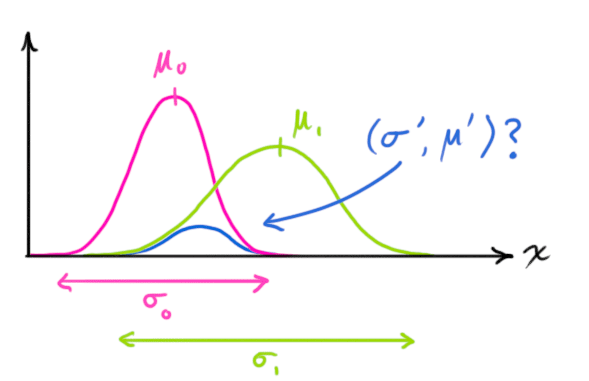
\includegraphics{gauss_joint.png}
\caption{gauss joint}
\end{figure}

\end{frame}

\begin{frame}{}

\begin{itemize}
\tightlist
\item
  \(\mu’ = \mu_0 + \frac{\sigma_0^2 (\mu_1 – \mu_0)} {\sigma_0^2 + \sigma_1^2}\)
\item
  \({\sigma’}^2 = \sigma_0^2 – \frac{\sigma_0^4} {\sigma_0^2 + \sigma_1^2}\)
\end{itemize}

\begin{figure}
\centering
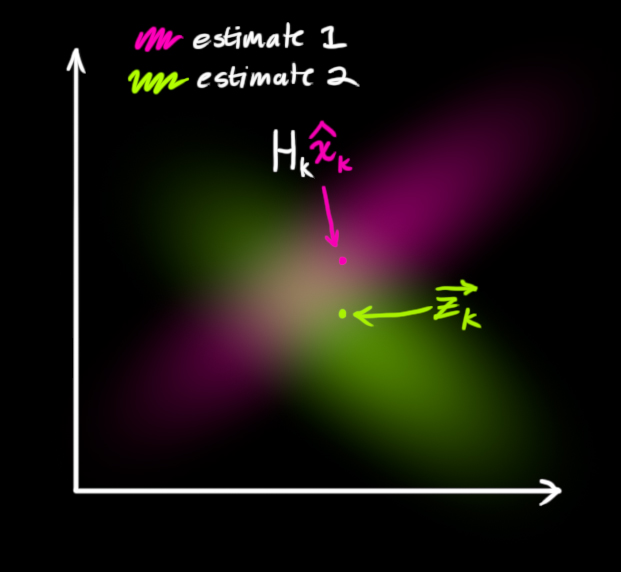
\includegraphics{combine.jpg}
\caption{combine}
\end{figure}

\end{frame}

\begin{frame}{Update}

\begin{itemize}
\tightlist
\item
  \(\mathbf{H}_t\) is the obs matrix (obs to state mapping)
\item
  Innovation or measurement residual:
  \(\tilde{\mathbf{y}}_t = \mathbf{z}_t - \mathbf{H}_t\hat{\mathbf{x}}_{t\mid t-1}\)
\item
  Innovation covariance:
  \(\mathbf{S}_t = \mathbf{H}_t \mathbf{P}_{t\mid t-1} \mathbf{H}_t^\mathrm{T} + \mathbf{R}_t\)
\item
  Optimal Kalman gain:
  \(\mathbf{K}_t = \mathbf{P}_{t\mid t-1}\mathbf{H}_t^\mathrm{T} \mathbf{S}_t^{-1}\)
\item
  Updated (a posteriori) state estimate:
  \(\hat{\mathbf{x}}_{t\mid t} = \hat{\mathbf{x}}_{t\mid t-1} + \mathbf{K}_t\tilde{\mathbf{y}}_t\)
\item
  Updated (a posteriori) estimate covariance
  \(\mathbf{P}_{t|t} = (\mathbf{I} - \mathbf{K}_t \mathbf{H}_t) \mathbf{P}_{t|t-1}\)
  \textbar{}\}
\end{itemize}

\end{frame}

\begin{frame}{}

\begin{figure}
\centering
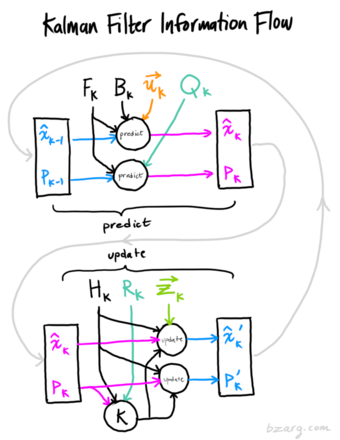
\includegraphics{kalflow.png}
\caption{Kalman filter flow}
\end{figure}

\end{frame}

\begin{frame}{}

The random variables we are interested in here are:

\begin{itemize}
\tightlist
\item
  \textbf{position} (x, y, z)
\item
  \textbf{attitude} (orientation)
\item
  \textbf{velocity}
\item
  \textbf{angular velocity}
\item
  \textbf{sensor biases}
\item
  Earth magnetic field components
\end{itemize}

(In bold the ones I will focus on for this project)

\end{frame}

\begin{frame}{}

The observations can come under many form:

\begin{itemize}
\tightlist
\item
  \textbf{motion capture systems like Vicon} (output relative position
  from 6 cameras around the lab tracking some markers)
\item
  \textbf{acceleratometer} (for linear velocity)
\item
  \textbf{gyroscope} (for angular velocity)
\item
  magnetometer
\item
  GPS
\item
  Optical flow (camera with some points as referentials)
\item
  LIDAR for altitude or cloudpoints
\end{itemize}

(In bold the ones I will focus on for this project)

\end{frame}

\begin{frame}{Non-linearity}

Rotations are non-linear operations so we cannot just apply vanilla KF.

Because \(Cov(f(X))\) for an arbitrary f has no closed form solution.

\textbf{Differentiation to the rescue!}

\end{frame}

\begin{frame}{Extended Kalman Filter}

Extended Kalman filter are an extension of kalman filters for
\textbf{non linear systems}.

F and H are linearized by an approximation of the first order using
Jacobians:

\begin{itemize}
\tightlist
\item
  \(\hat{\boldsymbol{x}}_{k|k-1} = f(\hat{\boldsymbol{x}}_{k-1|k-1}, \boldsymbol{u}_{k-1})\)
\item
  \(\tilde{\boldsymbol{y}}_{k} = \boldsymbol{z}_{k} - h(\hat{\boldsymbol{x}}_{k|k-1})\)
\item
  \({{\boldsymbol{F}_{k-1}}} = \left . \frac{\partial f}{\partial \boldsymbol{x} } \right \vert _{\hat{\boldsymbol{x}}_{k-1|k-1},\boldsymbol{u}_{k-1}}\)
\item
  \({{\boldsymbol{H}_{k}}} = \left . \frac{\partial h}{\partial \boldsymbol{x} } \right \vert _{\hat{\boldsymbol{x}}_{k|k-1}}\)
\end{itemize}

\end{frame}

\begin{frame}{Quaternions (optional)}

Quaternions are an extensions of complex numbers but with 2 extra
dimensions \[i^2=j^2=j^2=ijk=-1\]

Unit quaternions, also known as versors, can be used to represent
orientations and rotations in 3D.

Compared to Euler Angles, they are easier to compose and avoid gimbal
lock.

\end{frame}

\section{Extensions}\label{extensions}

\begin{frame}{Parralelizable, Pipelinable ?}

Matrixes involved are small and some known in advance.

Unrolling and parralelizing potential to shorten latency time.

Investigate theorotical implication of pipelining by using
\[\mathbf{X}_{t|t-k}\] with k the length of the pipeline.

\end{frame}

\begin{frame}{Other applications}

\begin{itemize}
\tightlist
\item
  VR headsets also include an IMU whose reactivity is crucial for
  immersion
\item
  Not only drones but the whole field of robotic use kalman filter for
  various planning tasks.
\end{itemize}

\end{frame}
